\documentclass[]{IEEEtran}
% Your packages go here
\usepackage[utf8]{inputenc}
\usepackage{graphicx}
\usepackage{grffile}
\usepackage{gensymb}
\usepackage{amsmath}
\usepackage{amssymb}
\usepackage{listings}
\usepackage{mathtools}
\usepackage{subfig}
\usepackage{xcolor}
\usepackage{multirow}
\usepackage{xfrac}
\usepackage{amsmath}
\usepackage{float}
\DeclareMathOperator{\atantwo}{atan2}

\DeclareMathOperator{\arctantwo}{arctan2}


\definecolor{codegreen}{rgb}{0,0.6,0}
\definecolor{codegray}{rgb}{0.5,0.5,0.5}
\definecolor{codepurple}{rgb}{0.58,0,0.82}
\definecolor{backcolour}{rgb}{0.95,0.95,0.92}

\lstdefinestyle{mystyle}{
    backgroundcolor=\color{backcolour},   
    commentstyle=\color{codegreen},
    keywordstyle=\color{magenta},
    numberstyle=\tiny\color{codegray},
    stringstyle=\color{codepurple},
    basicstyle=\ttfamily\footnotesize,
    breakatwhitespace=false,         
    breaklines=true,                 
    captionpos=b,                    
    keepspaces=true,                 
    numbers=left,                    
    numbersep=5pt,                  
    showspaces=false,                
    showstringspaces=false,
    showtabs=false,                  
    tabsize=2
}
 
\lstset{style=mystyle}
 
\usepackage{lipsum}% http://ctan.org/pkg/lipsum
\usepackage{graphicx}% http://ctan.org/pkg/graphicx

\def\footnoterule{\relax%
  \kern-2pt
  \hbox to \columnwidth{\hfill\vrule width 0.7\columnwidth height 0.4pt\hfill}
  \kern4.6pt}
\makeatother

\renewcommand{\lstlistingname}{Algorithm}% Listing -> Algorithm
\usepackage[noadjust]{cite}
\markboth{MO433 - Unsupervised Machine Learning }{}

%\usepackage{graphicx}
%\graphicspath{{../output/}}

\begin{document}

\title{Project 2 }
\author{Ivan Lima do Espirito Santo \thanks{RA: 956694 - i956694@g.unicamp.br}\\ Rosa Yuliana Gabriela Paccotacya Yanque \thanks{RA: 263068 - r263068@dac.unicamp.br} \\ Thiago Gomes Marçal Pereira \thanks{RA: 189691 - t189691@g.unicamp.br}}

\maketitle
%%\begin{abstract}
%%\end{abstract}

\section{Project Description}
Learning effective visual representations without human supervision is a long-standing problem. Most mainstream approaches fall into one of two classes: 
\begin{itemize}
    \item generative that learn to model the input distribution
    \item discriminative that learn splitting hyperplanes to distinguish the classes. 
\end{itemize}
Inspired by recent contrastive learning algorithms, SimCLR~\cite{chen2020simple} learns representations by maximizing agreement between differently augmented views of the same data example via a contrastive loss in the latent space. 

\section{Goal}\label{simCLR}
The goal of this project is to reproduce the results of SimCLR~\cite{chen2020simple} for CIFAR10. In other words, implementing SimCLR's method and execute the experiments to compare: 
\begin{itemize}
    \item different augmentation functions T
    \item different similarity functions
\end{itemize}
We intent to experiment with different architecture's configurations (beyond the one presented in the paper) and perform further comparison. 
In order to do so, we evaluate different transformation functions T to augment the data (section 3,~\cite{chen2020simple}) and then compare their performance. As well, Chen et al. use the cosine similarity as their main similarity function. We  evaluate other similarities and explore how they change the method’s performance. 
Regarding their architecture for the encoder \(f(·)\)  and the projection head \(g(·)\), 

we use their proposal 

we use a reduced version of their proposal, so we can train it. 

we radically changed their architectures 

(See Fig.~\ref{fig01} for a graphical representation.) 
We explain the architecture in more details in the results session. 
\begin{figure}[!h]
\centering
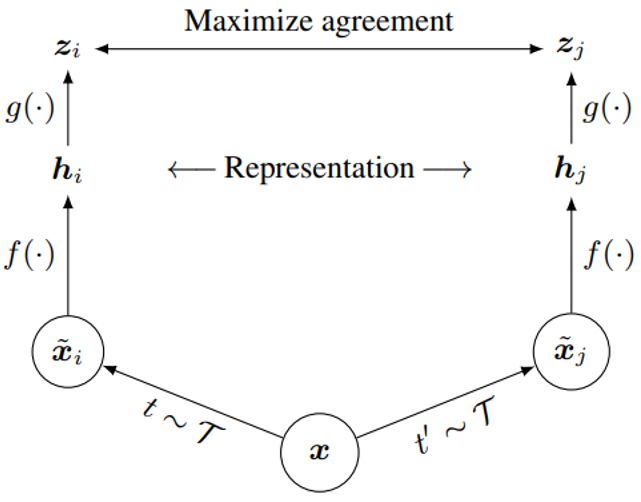
\includegraphics[width=9cm]{home/MO433A/proj02/images/fluxSimCLS.PNG}
\caption{SimCLR [~\cite{chen2020simple}, Fig. 2] framework. Two separate data augmentation operators are sampled from the same family of augmentations and applied to each data example to obtain two correlated views. A base encoder network $f(\cdot)$ and a projection head $g(\cdot)$ are trained to maximize agreement using a contrastive loss. After training is completed, we throw away the projection head $g(\cdot)$ and use encoder $f(\cdot)$ and representation h for downstream tasks}
\label{fig01}
\end{figure}


\section{SimCLR Introduction}
SimCLR presents a simple framework for contrastive learning of visual representations. They simplify recently proposed contrastive selfsupervised learning algorithms without requiring specialized architectures or a memory bank. In order to understand what enables the contrastive prediction tasks to learn useful representations, they systematically study the major components of their framework. They show that (1) composition of data augmentations plays a critical role in defining effective predictive tasks, (2) introducing a learnable nonlinear transformation between the representation and the contrastive loss substantially improves the quality of the learned representations, and (3) contrastive learning benefits from larger batch sizes and more training steps compared to supervised learning. By combining these findings, they were able to considerably outperform previous methods for self-supervised and semi-supervised learning on ImageNet. A linear classifier trained on self-supervised representations learned by SimCLR achieves $76.5 \%$ top-1 accuracy, which is a $7\%$ relative improvement over previous state-of-the-art, matching the performance of a supervised ResNet-50. When fine-tuned on only $1\%$ of the labels, they achieved $85.8 \%$ top-5 accuracy, outperforming AlexNet with $100 \times$ fewer labels.

\section{SimCLR Overview}
In this work, we introduce a simple framework for contrastive learning of visual representations, which we call SimCLR. Not only does SimCLR outperform previous work, but it is also simpler, requiring neither specialized architectures nor a memory bank. In order to understand what enables good contrastive representation learning, we systematically study the major components of our framework and show that: 
\begin{itemize}
    \item Composition of multiple data augmentation operations is crucial in defining the contrastive prediction tasks that 
    \item Introducing a learnable nonlinear transformation between the representation and the contrastive loss substantially improves the quality of the learned representations.
    \item Representation learning with contrastive cross entropy loss benefits from normalized embeddings and an appropriately adjusted temperature parameter.
    \item Contrastive learning benefits from larger batch sizes and longer training compared to its supervised counterpart. Like supervised learning, contrastive learning benefits from deeper and wider networks.
\end{itemize}

We combine these findings to achieve a new state-of-the-art in self-supervised and semi-supervised learning on ImageNet ILSVRC-2012 (Russakovsky et al., 2015). Under the linear evaluation protocol, SimCLR achieves $76.5 \%$ top-1 accuracy, which is a $7 \%$ relative improvement over previous state-of-the-art (Hénaff et al., 2019). When fine-tuned with only $1 \%$ of the ImageNet labels, SimCLR achieves $85.8 \%$ top-5 accuracy, a relative improvement of $10 \%$ (Hénaff et al., 2019 ). When fine-tuned on other natural image classification datasets, SimCLR performs on par with or better than a strong supervised baseline (Kornblith et al., 2019 ) on 10 out of 12 datasets.


\section{SimCLR Method}
\subsection{The Contrastive Learning Framework}

Inspired by recent contrastive learning algorithms (see Section $7 \text { for an overview }),$ SimCLR learns representations by maximizing agreement between differently augmented views of the same data example via a contrastive loss in the latent space. As illustrated in Figure $2,$ this framework comprises the following four major components.

\begin{itemize}
    \item A stochastic data augmentation module that transforms any given data example randomly resulting in two correlated views of the same example, denoted $\tilde{x}_{i}$ and $\tilde{x}_{j}$ which we consider as a positive pair. In this work, we sequentially apply three simple augmentations: random cropping followed by resize back to the original size, random color distortions, and random Gaussian blur. As shown in Section $3,$ the combination of random crop and color distortion is crucial to achieve a good performance.
    \item A neural network base encoder $f(\cdot)$ that extracts representation vectors from augmented data examples. Our framework allows various choices of the network architecture without any constraints. We opt for simplicity and adopt the commonly used ResNet (He et al., 2016) to obtain $\boldsymbol{h}_{i}=f\left(\tilde{\boldsymbol{x}}_{i}\right)=\operatorname{ResNet}\left(\tilde{\boldsymbol{x}}_{i}\right)$ where $\boldsymbol{h}_{i} \in \mathbb{R}^{d}$ is the output after the average pooling layer.
    
     \item A small neural network projection head $g(\cdot)$ that maps representations to the space where contrastive loss is applied. We use a MLP with one hidden layer to obtain $z_{i}=g\left(\boldsymbol{h}_{i}\right)=W^{(2)} \sigma\left(W^{(1)} \boldsymbol{h}_{i}\right)$ where $\sigma$ is a ReLU non-
linearity. As shown in section $4,$ we find it beneficial to define the contrastive loss on $z_{i}$ 's rather than $h_{i}$ 's.
     \item A contrastive loss function defined for a contrastive prediction task. Given a set $\left\{\tilde{\boldsymbol{x}}_{k}\right\}$ including a positive pair of examples $\tilde{x}_{i}$ and $\tilde{x}_{j},$ the contrastive prediction task aims to identify $\tilde{x}_{j}$ in $\left\{\tilde{x}_{k}\right\}_{k \neq i}$ for a given $\tilde{x}_{i}$
\end{itemize}
We randomly sample a minibatch of $N$ examples and define the contrastive prediction task on pairs of augmented examples derived from the minibatch, resulting in $2 N$ data points. We do not sample negative examples explicitly. Instead, given a positive pair, similar to (Chen et al., 2017 ), we treat the other $2(N-1)$ augmented examples within a minibatch as negative examples. Let $\operatorname{sim}(\boldsymbol{u}, \boldsymbol{v})=\boldsymbol{u}^{\top} \boldsymbol{v} /\|\boldsymbol{u}\|\|\boldsymbol{v}\|$ de-
note the cosine similarity between two vectors $u$ and $v$ Then the loss function for a positive pair of examples $(i, j)$ is defined as: 

\begin{equation}
\ell_{i, j}=-\log \frac{\exp \left(\operatorname{sim}\left(z_{i}, z_{j}\right) / \tau\right)}{\sum_{k=1}^{2 N} \mathbb{1}_{[k \neq i]} \exp \left(\operatorname{sim}\left(z_{i}, z_{k}\right) / \tau\right)}
\label{eq01}
\end{equation}

where $\mathbb{1}_{[k \neq i]} \in\{0,1\}$ is an indicator function evaluating to 1 iff $k \neq i$ and $\tau$ denotes a temperature parameter. The final loss is computed across all positive pairs, both $(i, j)$ and $(j, i),$ in a mini-batch. This loss has been used in previous work (Sohn, 2016; Wu et al., 2018; Oord et al., 2018 ; for convenience, we term it $N T$ -Xent (the normalized temperature-scaled cross entropy loss.
The following Algorithm summarizes the proposed method.


\begin{figure}[h!]
    \centering
    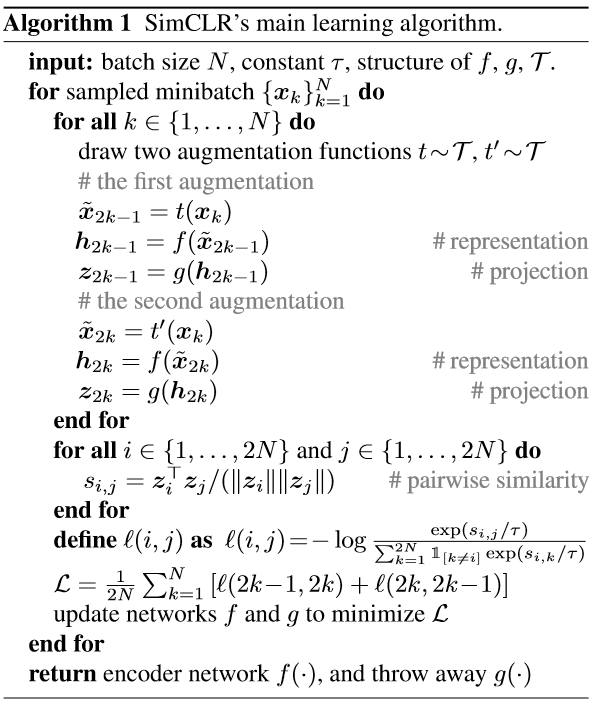
\includegraphics[width=9cm]{./images/psdocode.PNG}
%%    \caption{ }
    \label{psdocode}
\end{figure}


\subsection{Training with Large Batch Size}

We do not train the model with a memory bank (Wu et al., 2018 ). Instead, we vary the training batch size $N$ from 256 to $8192 .$ A batch size of 8192 gives us 16382 negative examples per positive pair from both augmentation views. Training with large batch size may be unstable when using standard SGD/Momentum with linear learning rate scaling (Goyal et al., 2017 ). To stabilize the training, we use the LARS optimizer (You et al., 2017 ) for all batch sizes.We train our model with Cloud TPUs, using 32 to 128 cores depending on the batch size. $^{2}$

Global BN. Standard ResNets use batch normalization (Ioffe \& Szegedy, 2015). In distributed training with data parallelism, the BN mean and variance are typically aggregated locally per device. In our contrastive learning, as positive pairs are computed in the same device, the model can exploit the local information leakage to improve prediction accuracy without improving representations. We address this issue by aggregating BN mean and variance over all devices during the training. Other approaches include shuffling data examples (He et al., 2019 ), or replacing BN with layer norm (Hénaff et al., 2019).

\subsection{Evaluation Protocol}

Here we lay out the protocol for our empirical studies, which aim to understand different design choices in our framework.

\begin{figure}[!ht]
  \centering
  \subfloat[Global and Local Views]{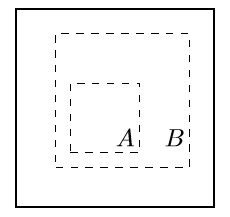
\includegraphics[width=0.22\textwidth]{./images/fig3_a}}
  \hspace{1mm}
  \subfloat[Adjacent Views]{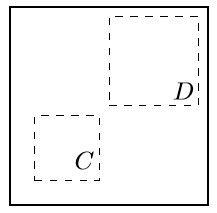
\includegraphics[width=0.22\textwidth]{images/fig3_b}}
  \hspace{1mm}
  \break
  \caption{Solid rectangles are images, dashed rectangles are random crops. By randomly cropping images, we sample contrastive prediction tasks that include global to local view $(B \rightarrow A)$ or adjacent view $(D \rightarrow C)$ prediction. }
  \label{fig3}
\end{figure}

Dataset and Metrics. Most of our study for unsupervised pretraining (learning encoder network $f$ without labels) is done using the ImageNet ILSVRC-2012 dataset (Russakovsky et al., 2015 ). Some additional pretraining experiments on CIFAR-10 (Krizhevsky \& Hinton, 2009) can be found in Appendix B.9. We also test the pretrained results on a wide range of datasets for transfer learning. To evaluate the learned representations, we follow the widely used linear evaluation protocol (Zhang et al., $2016 ;$ Oord et al. $2018 ;$ Bachman et al., $2019 ;$ Kolesnikov et al., 2019 , where
a linear classifier is trained on top of the frozen base network, and test accuracy is used as a proxy for representation quality. Beyond linear evaluation, we also compare against state-of-the-art on semi-supervised and transfer learning.
Default setting. Unless otherwise specified, for data augmentation we use random crop and resize (with random flip), color distortions, and Gaussian blur (for details, see Appendix A). We use ResNet-50 as the base encoder network, and a 2 -layer MLP projection head to project the representation to a 128 -dimensional latent space. As the loss, we use NT-Xent, optimized using LARS with linear learning rate scaling (i.e. LearningRate $=0.3 \times$ BatchSize $/ 256$ ) and weight decay of $10^{-6}$. We train at batch size 4096 for 100 epochs. $^{3}$ Furthermore, we use linear warmup for the first 10 epochs, and decay the learning rate with the cosine decay schedule without restarts (Loshchilov \& Hutter, 2016).

\section{Data Augmentation for Contrastive Representation Learning }

Data augmentation defines predictive tasks. While data augmentation has been widely used in both supervised and unsupervised representation learning (Krizhevsky et al. $2012 ;$ Hénaff et al., $2019 ;$ Bachman et al., 2019 , it has not been considered as a systematic way to define the contrastive prediction task. Many existing approaches define contrastive prediction tasks by changing the architecture.

\begin{figure}[!ht]
  \centering
  \subfloat[Original]{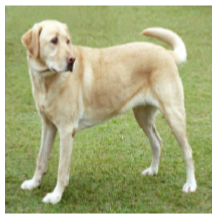
\includegraphics[width=0.19\textwidth]{./images/fig4_a}}
  \hspace{1mm}
  \subfloat[Crop and Resize]{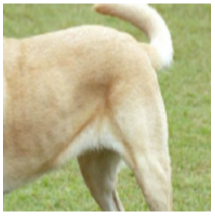
\includegraphics[width=0.19\textwidth]{images/fig4_b}}
  \hspace{1mm}
  \subfloat[Crop, resize and flip]{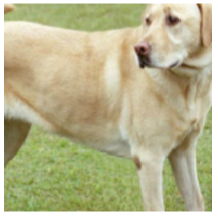
\includegraphics[width=0.19\textwidth]{images/fig4_c}}
  \hspace{1mm}
  \subfloat[Color dist drop]{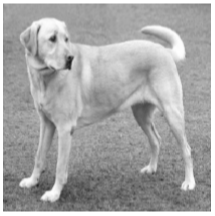
\includegraphics[width=0.19\textwidth]{images/fig4_d}}
  \hspace{1mm}
  \subfloat[Color dist jitter]{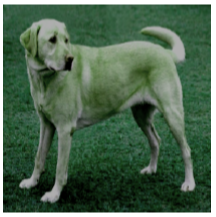
\includegraphics[width=0.19\textwidth]{images/fig4_e}}
  \hspace{1mm}
 \break %%%%%%%%%%%
  \subfloat[Rotate]{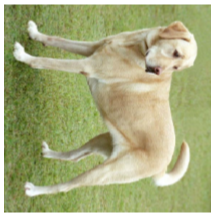
\includegraphics[width=0.19\textwidth]{images/fig4_f}}
  \hspace{1mm}
  \subfloat[Cutout]{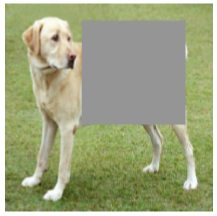
\includegraphics[width=0.19\textwidth]{images/fig4_g}}
  \hspace{1mm}
  \subfloat[Gaussian noise]{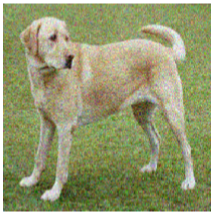
\includegraphics[width=0.19\textwidth]{images/fig4_h}}
  \hspace{1mm}
  \subfloat[i]{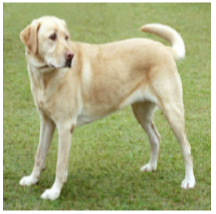
\includegraphics[width=0.19\textwidth]{images/fig4_i}}
  \hspace{1mm}
  \subfloat[Sobel Filtering]{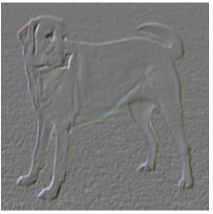
\includegraphics[width=0.19\textwidth]{images/fig4_j}}
  \hspace{1mm}
  \caption{Illustrations of the studied data augmentation operators. Each augmentation can transform data stochastically with some internal parameters (e.g. rotation degree, noise level). Note that we only test these operators in ablation, the augmentation policy used to train our models only includes random crop (with flip and resize), color distortion, and Gaussian blur. (Original image cc-by: Von.grzanka) }
  \label{fig4}
\end{figure}

For example, Hjelm et al. (2018)$;$ Bachman et al. (2019) achieve global-to-local view prediction via constraining the receptive field in the network architecture, whereas Oord et al. (2018)$;$ Hénaff et al. (2019) achieve neighboring view prediction via a fixed image splitting procedure and a context aggregation network. We show that this complexity can be avoided by performing simple random cropping (with resizing of target images, which creates a family of predictive tasks subsuming the above mentioned two, as shown in Figure
3. This simple design choice conveniently decouples the predictive task from other components such as the neural network architecture. Broader contrastive prediction tasks can be defined by extending the family of augmentations and composing them stochastically.

\subsection{Composition of data augmentation operations is crucial for learning good representations }
To systematically study the impact of data augmentation, we consider several common augmentations here. One type of augmentation involves spatial/geometric transformation of data, such as cropping and resizing (with horizontal flipping), rotation (Gidaris et al., 2018 ) and cutout (DeVries \& Taylor, 2017). The other type of augmentation involves appearance transformation, such as color distortion (including color dropping, brightness, contrast, saturation, hue) (Howard, $2013 ;$ Szegedy et al., 2015 ), Gaussian blur, and Sobel filtering. Figure 4 visualizes the augmentations that we study in this work.

To understand the effects of individual data augmentations and the importance of augmentation composition, we investigate the performance of our framework when applying

\begin{figure}[!h]
    \centering
    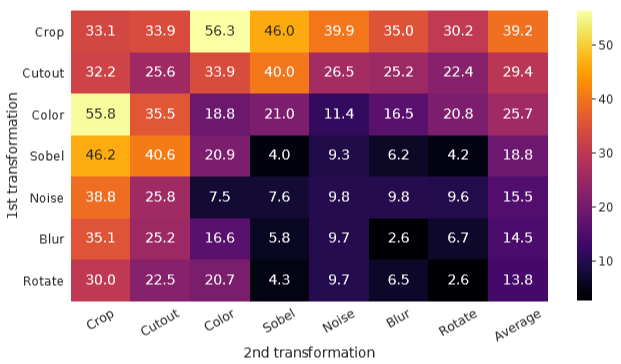
\includegraphics[width=9cm]{images/fig5.PNG}
    \caption{Linear evaluation (ImageNet top-1 accuracy) under individual or composition of data augmentations, applied only to one branch. For all columns but the last, diagonal entries correspond to single transformation, and off-diagonals correspond to composition of two transformations (applied sequentially). The last column reflects the average over the row.}
    \label{fig5}
\end{figure}

augmentations individually or in pairs. since ImageNet images are of different sizes, we always apply crop and resize images (Krizhevsky et al., 2012; Szegedy et al., 2015), which makes it difficult to study other augmentations in the absence of cropping. To eliminate this confound, we consider an asymmetric data transformation setting for this ablation. Specifically, we always first randomly crop images and resize them to the same resolution, and we then apply the targeted transformation(s) only to one branch of the framework in Figure $2,$ while leaving the other branch as the identity (i.e. $t\left(x_{i}\right)=x_{i}$ ). Note that this asymmetric data augmentation hurts the performance. Nonetheless, this setup should not substantively change the impact of individual data augmentations or their compositions.

\begin{figure}[!h]
  \centering
  \subfloat[Without color distortion]{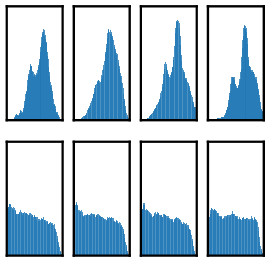
\includegraphics[width=0.22\textwidth]{./images/fig6_a.PNG}}
  \hspace{1mm}
  \subfloat[With color distortion]{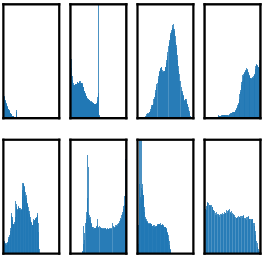
\includegraphics[width=0.22\textwidth]{images/fig6_b.PNG}}
  \hspace{1mm}
  \break
  \caption{Histograms of pixel intensities (over all channels) for different crops of two different images (i.e. two rows). The image for the first row is from figure ~\ref{fig4} All axes have the same range.}
  \label{fig6}
\end{figure}


\begin{table}[h!]
\caption{ Top-1 accuracy of unsupervised ResNet-50 using linear evaluation and supervised ResNet- $50^{5}$, under varied color distortion strength (see Appendix A) and other data transformations. Strength $1(+\text { Blur })$ is our default data augmentation policy.}
\label{table1}
\begin{tabular}{l|ccccc|c}
\hline & \multicolumn{4}{|c|} { Color distortion strength } & \\
Methods & $1 / 8$ & $1 / 4$ & $1 / 2$ & 1 & $1(+\text { Blur })$ & AutoAug \\
\hline SimCLR & 59.6 & 61.0 & 62.6 & 63.2 & 64.5 & 61.1 \\
Supervised & 77.0 & 76.7 & 76.5 & 75.7 & 75.4 & 77.1 \\
\hline
\end{tabular}
\end{table}

Figure~\ref{fig5} shows linear evaluation results under individual and composition of transformations. We observe that no single transformation suffices to learn good representations, even though the model can almost perfectly identify the positive pairs in the contrastive task. When composing augmentations, the contrastive prediction task becomes harder, but the quality of representation improves dramatically.
One composition of augmentations stands out: random cropping and random color distortion. We conjecture that one serious issue when using only random cropping as data augmentation is that most patches from an image share a similar color distribution. Figure 6 shows that color histograms alone suffice to distinguish images. Neural nets may exploit this shortcut to solve the predictive task. Therefore, it is critical to compose cropping with color distortion in order to learn generalizable features.

\subsection{Contrastive learning needs stronger data augmentation than supervised learning}
 
 To further demonstrate the importance of the color augmentation, we adjust the strength of color augmentation as shown in Table $1 .$ Stronger color augmentation substantially improves the linear evaluation of the learned unsupervised models. In this context, AutoAugment (Cubuk et al. 2019 , a sophisticated augmentation policy found using supervised learning, does not work better than simple cropping
$+(\text { stronger })$ color distortion. When training supervised models with the same set of augmentations, we observe that stronger color augmentation does not improve or even hurts their performance. Thus, our experiments show that unsupervised contrastive learning benefits from stronger (color) data augmentation than supervised learning. Although previous work has reported that data augmentation is useful for self-supervised learning (Doersch et al., 2015 ; Bachman et al., $2019 ;$ Hénaff et al., $2019 ;$ Asano et al., 2019 ), we show that data augmentation that does not yield accuracy benefits for supervised learning can still help considerably with contrastive learning.
 
 \begin{figure}[!h]
    \centering
    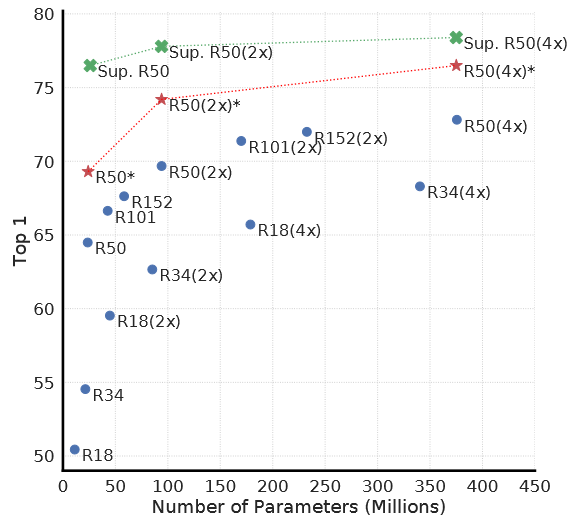
\includegraphics[width=9cm]{images/fig7.PNG}
    \caption{Linear evaluation of models with varied depth and width. Models in blue dots are ours trained for 100 epochs, models in red stars are ours trained for 1000 epochs, and models in green crosses are supervised ResNets trained for 90 epochs' (He et al., 2016).}
\label{fig7}
\end{figure}
 
\section{Architectures for Encoder and Head}
 
\subsection{Unsupervised contrastive learning benefits(more) from bigger models }

Figure~\ref{fig7} shows, perhaps unsurprisingly, that increasing depth and width both improve performance. While similar findings hold for supervised learning (He et al., 2016 ), we find the gap between supervised models and linear classifiers trained on unsupervised models shrinks as the model size increases, suggesting that unsupervised learning benefits more from bigger models than its supervised counterpart.

\subsection{A nonlinear projection head improves the representation quality of the layer before it }

We then study the importance of including a projection head, i.e. $g(h) .$ Figure 8 shows linear evaluation results

\begin{figure}[!h]
\centering
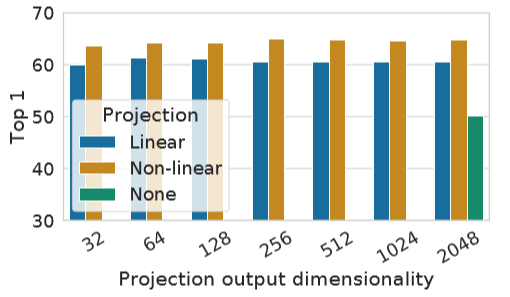
\includegraphics[width=9cm]{images/fig8.PNG}
\caption{Linear evaluation of representations with different projection heads go and various dimensions of $z = g(h)$. The representation h (before projection) is 2048-dimensional here.}
\label{fig8}
\end{figure}

\begin{table}[!ht]
\caption{Accuracy of training additional MLPs on different representations to predict the transformation applied. Other than crop and color augmentation, we additionally and independently add rotation (one of $\left\{0^{\circ}, 90^{\circ}, 180^{\circ}, 270^{\circ}\right\}$ ), Gaussian noise, and So bel filtering transformation during the pretraining for the last three rows. Both $h$ and $g(h)$ are of the same dimensionality, i.e. 2048}
\label{table3}
\begin{tabular}{lccc}
\hline What to predict? & Random guess & Representation $\boldsymbol{h}$ & $g(\boldsymbol{h})$ \\
\hline Color vs grayscale & 80 & 99.3 & 97.4 \\
Rotation & 25 & 67.6 & 25.6 \\
Orig. vs corrupted & 50 & 99.5 & 59.6 \\
Orig. vs Sobel filtered & 50 & 96.6 & 56.3 \\
\hline
\end{tabular}
\end{table}

\subsection{Loss Functions and Batch Size}
\subsubsection{Normalized cross entropy loss with adjustable temperature works better than alternatives }
\subsubsection{Contrastive learning benefits(more) from larger batch sizes and longer training}
\subsection{Comparison with State-of-the-art and SimCLR Conclusion}

\section{Development Stages}

\begin{itemize}
    \item 
    \item 
    \item 
\end{itemize}

\section{Difficulties}

\section{Adopted Approach}

\section{Results}

\section{Conclusion}

\bibliographystyle{abbrv}
\bibliography{bibliography}

\clearpage
\onecolumn
\begin{appendices}

\section{SimCLR Tables and Benchmark} \label{sec:appendix-1}

\begin{table}[h!]
\caption{Negative loss functions and their gradients. All input vectors, i.e. $u, v^{+}, v^{-},$ are $\ell_{2}$ normalized. NT-Xent is an abbreviation for "Normalized Temperature-scaled Cross Entropy". Different loss functions impose different weightings of positive and negative examples}
\label{table2}
\begin{tabular}{c|c|c}
\hline Name & Negative loss function & Gradient w.r.t. $\boldsymbol{u}$ \\
\hline NT-Xent & $\boldsymbol{u}^{T} \boldsymbol{v}^{+} / \tau-\log \sum_{\boldsymbol{v} \in\left\{\boldsymbol{v}^{+}, \boldsymbol{v}^{-}\right\}} \exp \left(\boldsymbol{u}^{T} \boldsymbol{v} / \tau\right)$ & $\left(1-\frac{\exp \left(\boldsymbol{u}^{T} \boldsymbol{v}^{+} / \tau\right)}{Z(\boldsymbol{u})}\right) / \tau \boldsymbol{v}^{+}-\sum_{\boldsymbol{v}^{-}} \frac{\exp \left(\boldsymbol{u}^{T} \boldsymbol{v}^{-} / \tau\right)}{Z(\boldsymbol{u})} / \tau \boldsymbol{v}^{-}$ \\
NT-Logistic & $\log \sigma\left(\boldsymbol{u}^{T} \boldsymbol{v}^{+} / \tau\right)+\log \sigma\left(-\boldsymbol{u}^{T} \boldsymbol{v}^{-} / \tau\right)$ & $\left(\sigma\left(-\boldsymbol{u}^{T} \boldsymbol{v}^{+} / \tau\right)\right) / \tau \boldsymbol{v}^{+}-\sigma\left(\boldsymbol{u}^{T} \boldsymbol{v}^{-} / \tau\right) / \tau \boldsymbol{v}^{-}$ \\
Margin Triplet & $-\max \left(\boldsymbol{u}^{T} \boldsymbol{v}^{-}-\boldsymbol{u}^{T} \boldsymbol{v}^{+}+m, 0\right)$ & $\boldsymbol{v}^{+}-\boldsymbol{v}^{-}$ if $\boldsymbol{u}^{T} \boldsymbol{v}^{+}-\boldsymbol{u}^{T} \boldsymbol{v}^{-}<m$ else $\mathbf{0}$ \\
\hline
\end{tabular}
\end{table}
 


\begin{tabular}{ccccc}
\hline Margin & NT-Logi. & Margin (sh) & NT-Logi.(sh) & NT-Xent \\
\hline 50.9 & 51.6 & 57.5 & 57.9 & 63.9 \\
\hline
\end{tabular}
Table
4. Linear evaluation (top-1) for models trained with different loss functions. "sh" means using semi-hard negative mining.

\begin{tabular}{cc|cc|c}
\hline$\ell_{2}$ norm? & $\tau$ & Entropy & Contrastive acc. & Top 1 \\
\hline \multirow{4}{*} { Yes } & 0.05 & 1.0 & 90.5 & 59.7 \\
& 0.1 & 4.5 & 87.8 & 64.4 \\
& 0.5 & 8.2 & 68.2 & 60.7 \\
& 1 & 8.3 & 59.1 & 58.0 \\
\hline \multirow{2}{*} { No } & 10 & 0.5 & 91.7 & 57.2 \\
& 100 & 0.5 & 92.1 & 57.0 \\
\hline
\end{tabular}
Table
5. Linear evaluation for models trained with different choices
of $\ell_{2}$ norm and temperature $\tau$ for $\mathrm{NT}$ -Xent loss. The contrastive
distribution is over 4096 examples

\begin{tabular}{llccc}
\hline Method & Architecture & Param. & Top 1 & Top 5 \\
\hline Methods using ResNet-50: & & & \\
Local Agg. & ResNet-50 & 24 & 60.2 & $-$ \\
MoCo & ResNet-50 & 24 & 60.6 & $-$ \\
PIRL & ResNet-50 & 24 & 63.6 & $-$ \\
CPC v2 & ResNet-50 & 24 & 63.8 & 85.3 \\
SimCLR (ours) & ResNet-50 & 24 & $\mathbf{6 9 . 3}$ & $\mathbf{8 9 . 0}$ \\
\hline Methods using other architectures: & & & \\
Rotation & RevNet-50 $(4 \times)$ & 86 & 55.4 & $-$ \\
BigBiGAN & RevNet-50 $(4 \times)$ & 86 & 61.3 & 81.9 \\
AMDIM & Custom-ResNet & 626 & 68.1 & $-$ \\
CMC & ResNet-50 $(2 \times)$ & 188 & 68.4 & 88.2 \\
MoCo & ResNet-50 $(4 \times)$ & 375 & 68.6 & $-$ \\
CPC v2 & ResNet-161 $(*)$ & 305 & 71.5 & 90.1 \\
SimCLR (ours) & ResNet-50 $(2 \times)$ & 94 & 74.2 & 92.0 \\
SimCLR (ours) & ResNet-50 $(4 \times)$ & 375 & $\mathbf{7 6 . 5}$ & $\mathbf{9 3 . 2}$ \\
\hline
\end{tabular}
Table
5. ImageNet accuracies of linear classifiers trained on repre
sentations learned with different self-supervised methods.

\begin{tabular}{llcc}
\hline & & \multicolumn{2}{l} { Label fraction } \\
Method & Architecture & $1 \%$ & $10 \%$ \\
& & \multicolumn{2}{c} { Top 5 } \\
\hline Supervised baseline & ResNet-50 & 48.4 & 80.4 \\
\hline Methods using other label-propagation: & & & \\
Pseudo-label & ResNet-50 & 51.6 & 82.4 \\
VAT+Entropy Min. & ResNet-50 & 47.0 & 83.4 \\
UDA (w. RandAug) & ResNet-50 & $-$ & 88.5 \\
FixMatch (w. RandAug) & ResNet-50 & $-$ & 89.1 \\
S4L (Rot+VAT+En. M.) & ResNet-50 $(4 \times)$ & $-$ & 91.2 \\
\hline \multicolumn{3}{l} { Methods using representation learning only: } \\
InstDisc & ResNet-50 & 39.2 & 77.4 \\
BigBiGAN & RevNet-50 $(4 \times)$ & 55.2 & 78.8 \\
PIRL & ResNet-50 & 57.2 & 83.8 \\
CPC v2 & ResNet-161 $(*)$ & 77.9 & 91.2 \\
SimCLR (ours) & ResNet-50 & 75.5 & 87.8 \\
SimCLR (ours) & ResNet-50 $(2 \times)$ & 83.0 & 91.2 \\
SimCLR (ours) & ResNet- $50(4 \times)$ & $\mathbf{8 5 . 8}$ & $\mathbf{9 2 . 6}$ \\
\hline
\end{tabular}
able $7 .$ ImageNet accuracy of models trained with few labe

\newpage
\section{SimCLR Pictures} \label{sec:appendix-2}
%%%%%%%%%%%%%%%%%%%%%%%%%%%%%%%%%%%%%%%%%%%%%
\begin{figure}
    \centering
    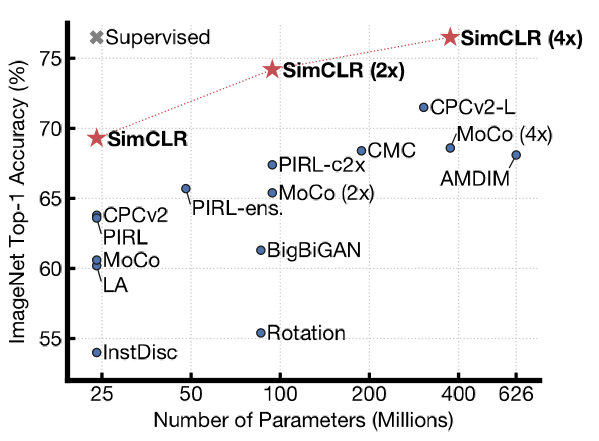
\includegraphics[width=9cm]{images/fig01_graph.PNG}
    \caption{ImageNet Top-1 accuracy of linear classifiers trained on representations learned with different self-supervised methods (pretrained on ImageNet). Gray cross indicates supervised ResNet-50. Our method, SimCLR, is shown in bold. }
    \label{fig1}
\end{figure}
%%%%%%%%%%%%%%%%%%%%%%%%%%%%%%%%%%%%%%%%%%%%%


%%%%%%%%%%%%%%%%%%%%%%%%%%%%%%%%%%%%%%%%%%%%%
\begin{figure}
    \centering
    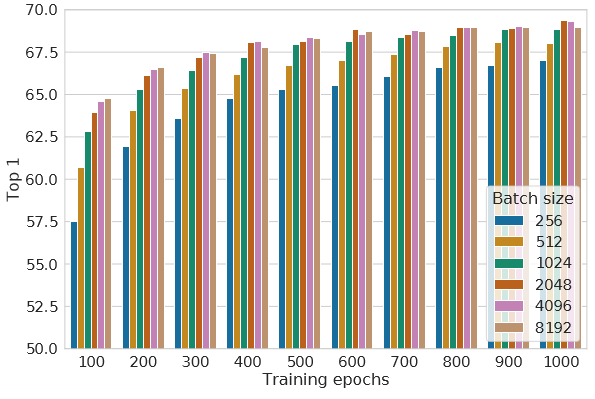
\includegraphics[width=9cm]{images/fig9.PNG}
    \caption{Linear evaluation models (ResNet-50) trained with different batch size and epochs. Each bar is a single run from scratch.}
    \label{fig9}
\end{figure}

%%%%%%%%%%%%%%%%%%%%%%%%%%%%%%%%%%%%%%%%%%%%%

\newpage
\end{appendices}
\end{document}